% Gemini theme
% https://github.com/anishathalye/gemini

\documentclass[final, 20pt]{beamer}

% ====================
% Packages
% ====================

\usepackage[T1]{fontenc}
\usepackage{lmodern}
\usepackage[size=custom,width=84.1,height=118.9,scale=1.0]{beamerposter}
\usetheme{gemini}
\usecolortheme{gemini}
\usepackage{graphicx}
\usepackage{booktabs}
\usepackage{tikz}
\usepackage{pgfplots}
\usepackage[square,sort,comma,numbers]{natbib}

% ====================
% Lengths
% ====================

% If you have N columns, choose \sepwidth and \colwidth such that
% (N+1)*\sepwidth + N*\colwidth = \paperwidth
\newlength{\sepwidth}
\newlength{\colwidth}
\setlength{\sepwidth}{0.025\paperwidth}
\setlength{\colwidth}{0.45\paperwidth}

\newcommand{\separatorcolumn}{\begin{column}{\sepwidth}\end{column}}

% ====================
% Title
% ====================

\title{The day-time patterns of carbohydrate intake in the UK adults \\ - results from the NDNS RP (2008-16)}

\author{Chaochen Wang \inst{1,2} \and Suzana Almoosawi \inst{3} \and Luigi Palla \inst{1}}

\institute[shortinst]{\inst{1} Dept Medical Statistics, LSHTM, London, UK; \samelineand \inst{2} Dept Public Health, Aichi Medical University, Aichi, Japan \samelineand \\ \inst{3} Brain, Performance and Nutrition Research Centre Northumbria University, Newcastle, UK}

% ====================
% Body
% ====================

\begin{document}

\begin{frame}[t]
\begin{columns}[t]
\separatorcolumn

\begin{column}{\colwidth}

  \begin{block}{Introduction}

The importance of the circadian rhythms has been recognized for long, while its impact on nutrition is still largely unknown. Meal timing has been found to be associated with a wide variety of physiological processes as well as health outcomes: 
    \vskip-1.45ex
    \begin{itemize}
	\item Skipping breakfast is associated with a higher risk of developing type 2 diabetes (T2D) \cite{uemura2015breakfast};
	\item While replacing fat at breakfast with carbohydrate is associated with lower risk of T2D incidence \cite{almoosawi2013diurnal};
	\item Evening intake of energy is positively associated with incidence of hypertension, and overweight/obesity \cite{Almoosawi2013,almoosawi2016chrono};
%	\item Shift workers have a higher risk of developing T2D \cite{pan2011rotating}. 
    \end{itemize}
    \vskip-1.45ex

Recent evidence suggested that there are three types of eaters \textbf{(grazers, early eaters, and later eaters)} according to the timing of energy consumption \cite{leech2017temporal,mansukhani2018investigating}. However, the temporal eating patterns were based only on averaging the total energy intake measured by one or two 24-hour dietary recalls and therefore \textbf{could not capture the day-to-day variation in eating patterns}, and \textbf{neither could it provide any clue of the temporal patterns specifically for nutrient intake}. This is mainly due to limitations in the dietary assessment methods (the questionnaires) often used in observational studies and the lack of understanding of statistical techniques that can capture and analyse the complexity of eating patterns across the day. 

This study aims at finding both time and quantity eating patterns specifically for carbohydrate (CH) intake in UK adults.

%    \begin{figure}
%      \centering
%      \begin{tikzpicture}[scale=6]
%        \draw[step=0.25cm,color=gray] (-1,-1) grid (1,1);
%        \draw (1,0) -- (0.2,0.2) -- (0,1) -- (-0.2,0.2) -- (-1,0)
%          -- (-0.2,-0.2) -- (0,-1) -- (0.2,-0.2) -- cycle;
%      \end{tikzpicture}
%      \caption{A figure caption.}
%    \end{figure}

%
%  \end{block}
%
%  \begin{block}{A block containing a list}



  \end{block}

%  \begin{alertblock}{A highlighted block}
%
%    This block catches your eye, so \textbf{important stuff} should probably go
%    here.
%
%    Curabitur eu libero vehicula, cursus est fringilla, luctus est. Morbi
%    consectetur mauris quam, at finibus elit auctor ac. Aliquam erat volutpat.
%    Aenean at nisl ut ex ullamcorper eleifend et eu augue. Aenean quis velit
%    tristique odio convallis ultrices a ac odio.
%
%    \begin{itemize}
%      \item \textbf{Fusce dapibus tellus} vel tellus semper finibus. In
%        consequat, nibh sed mattis luctus, augue diam fermentum lectus.
%      \item \textbf{In euismod erat metus} non ex. Vestibulum luctus augue in
%        mi condimentum, at sollicitudin lorem viverra.
%      \item \textbf{Suspendisse vulputate} mauris vel placerat consectetur.
%        Mauris semper, purus ac hendrerit molestie, elit mi dignissim odio, in
%        suscipit felis sapien vel ex.
%    \end{itemize}
%
%    Aenean tincidunt risus eros, at gravida lorem sagittis vel. Vestibulum ante
%    ipsum primis in faucibus orci luctus et ultrices posuere cubilia Curae.
%
%  \end{alertblock}

%\end{column}

%\separatorcolumn

%\begin{column}{\colwidth}
   \vskip-0.85ex
  \begin{block}{Data and Methodology}
    \vskip-1.45ex
\begin{itemize}
	\item Data from the National Diet and Nutrition Survey (NDNS) Rolling Programme (2008/09-15/16) included 6155 adults (2537 men and 3618 women) aged 19 or older in the UK. 
	\item Time of the day was categorized into 7 slots: 6-9 am, 9-12 noon, 12-2 pm, 2-5 pm, 5-8 pm, 8-10 pm and 10 pm-6 am. 
	\item Responses for CH intake within each time slot were categorised into: 1) no energy intake, 2) CH contributed $\geqslant$ 50\% or 3) CH contributed  $<$ 50\% of total energy. 
	\item Multilevel latent class analysis (MLCA) models\cite{finch2017multilevel} were applied to explore latent classes of CH consumption, accounting for the repeated measurement of intake on 3-4 days nested within individuals. 
	\item Survey-designed multivariable regression models were used to assess the associations of CH eating patterns with hypertension and obesity.
\end{itemize}
    \vskip-1.45ex


%    Vivamus congue volutpat elit non semper. Praesent molestie nec erat ac
%    interdum. In quis suscipit erat. \textbf{Phasellus mauris felis, molestie
%    ac pharetra quis}, tempus nec ante. Donec finibus ante vel purus mollis
%    fermentum. Sed felis mi, pharetra eget nibh a, feugiat eleifend dolor. Nam
%    mollis condimentum purus quis sodales. Nullam eu felis eu nulla eleifend
%    bibendum nec eu lorem. Vivamus felis velit, volutpat ut facilisis ac,
%    commodo in metus.
%
%    \begin{enumerate}
%      \item \textbf{Morbi mauris purus}, egestas at vehicula et, convallis
%        accumsan orci. Orci varius natoque penatibus et magnis dis parturient
%        montes, nascetur ridiculus mus.
%      \item \textbf{Cras vehicula blandit urna ut maximus}. Aliquam blandit nec
%        massa ac sollicitudin. Curabitur cursus, metus nec imperdiet bibendum,
%        velit lectus faucibus dolor, quis gravida metus mauris gravida turpis.
%      \item \textbf{Vestibulum et massa diam}. Phasellus fermentum augue non
%        nulla accumsan, non rhoncus lectus condimentum.
%    \end{enumerate}

  \end{block}



%  \begin{block}{Fusce aliquam magna velit}
%
%    Et rutrum ex euismod vel. Pellentesque ultricies, velit in fermentum
%    vestibulum, lectus nisi pretium nibh, sit amet aliquam lectus augue vel
%    velit. Suspendisse rhoncus massa porttitor augue feugiat molestie. Sed
%    molestie ut orci nec malesuada. Sed ultricies feugiat est fringilla
%    posuere.
%
%    \begin{figure}
%      \centering
%      \begin{tikzpicture}
%        \begin{axis}[
%            scale only axis,
%            no markers,
%            domain=0:2*pi,
%            samples=100,
%            axis lines=center,
%            axis line style={-},
%            ticks=none]
%          \addplot[red] {sin(deg(x))};
%          \addplot[blue] {cos(deg(x))};
%        \end{axis}
%      \end{tikzpicture}
%      \caption{Another figure caption.}
%    \end{figure}
%
%  \end{block}

%   \vskip-0.85ex
  \begin{block}{Day Level Carbohydrate Eating Patterns}
%\heading{Day Level Carbohydrate Eating Patterns}
      \vskip-2.45ex
    \begin{figure}
      \centering
      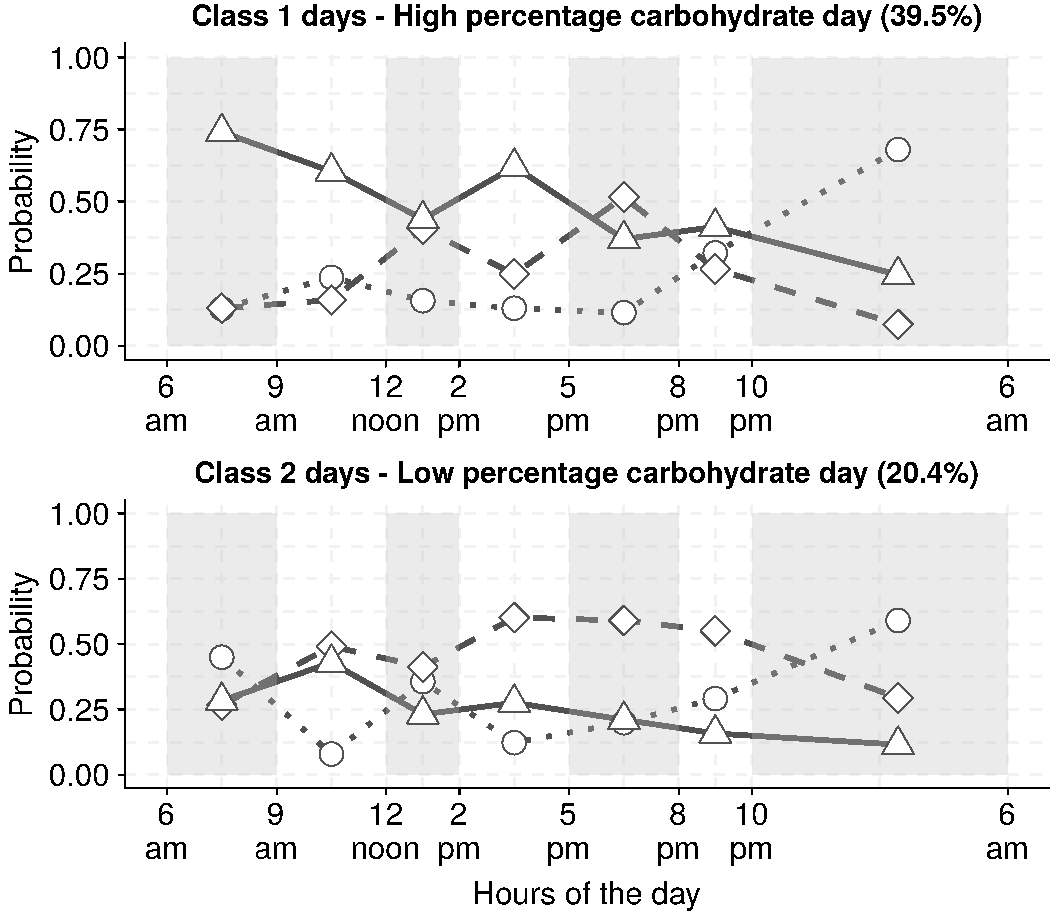
\includegraphics[width=30cm]{Fig/Fig01a.eps}
%      \caption{Day level latent class solutions (Class 1 and 2 days).}
    \end{figure}


%    Nulla eget sem quam. Ut aliquam volutpat nisi vestibulum convallis. Nunc a
%    lectus et eros facilisis hendrerit eu non urna. Interdum et malesuada fames
%    ac ante \textit{ipsum primis} in faucibus. Etiam sit amet velit eget sem
%    euismod tristique. Praesent enim erat, porta vel mattis sed, pharetra sed
%    ipsum. Morbi commodo condimentum massa, \textit{tempus venenatis} massa
%    hendrerit quis. Maecenas sed porta est. Praesent mollis interdum lectus,
%    sit amet sollicitudin risus tincidunt non.
%
%    Etiam sit amet tempus lorem, aliquet condimentum velit. Donec et nibh
%    consequat, sagittis ex eget, dictum orci. Etiam quis semper ante. Ut eu
%    mauris purus. Proin nec consectetur ligula. Mauris pretium molestie
%    ullamcorper. Integer nisi neque, aliquet et odio non, sagittis porta justo.
%
%    \begin{itemize}
%      \item \textbf{Sed consequat} id ante vel efficitur. Praesent congue massa
%        sed est scelerisque, elementum mollis augue iaculis.
%        \begin{itemize}
%          \item In sed est finibus, vulputate
%            nunc gravida, pulvinar lorem. In maximus nunc dolor, sed auctor eros
%            porttitor quis.
%          \item Fusce ornare dignissim nisi. Nam sit amet risus vel lacus
%            tempor tincidunt eu a arcu.
%          \item Donec rhoncus vestibulum erat, quis aliquam leo
%            gravida egestas.
%        \end{itemize}
%      \item \textbf{Sed luctus, elit sit amet} dictum maximus, diam dolor
%        faucibus purus, sed lobortis justo erat id turpis.
%      \item \textbf{Pellentesque facilisis dolor in leo} bibendum congue.
%        Maecenas congue finibus justo, vitae eleifend urna facilisis at.
%    \end{itemize}

  \end{block}



%  \begin{block}{A block containing some math}
%
%    Nullam non est elit. In eu ornare justo. Maecenas porttitor sodales lacus,
%    ut cursus augue sodales ac.
%
%    $$
%    \int_{-\infty}^{\infty} e^{-x^2}\,dx = \sqrt{\pi}
%    $$
%  \end{block}

\end{column}

\separatorcolumn

\begin{column}{\colwidth}

  \begin{block}

%  \begin{block}{Day Level Carbohydrate Eating Patterns}
	\vskip-2.45ex
	\begin{figure}
		\centering
		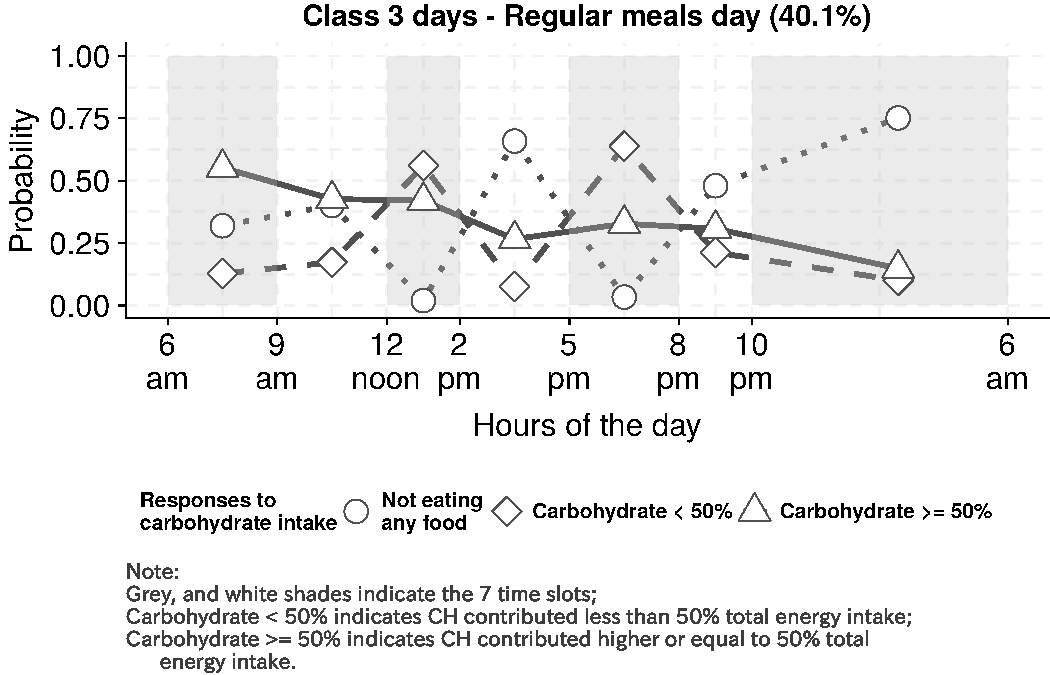
\includegraphics[width=33cm]{Fig/Fig01b.eps}	\vskip-2.45ex
		\caption{Day level latent class solutions (Three types of CH eating days).}
	\end{figure}
\vskip-1.80ex

  \end{block}


\vskip-2.45ex
  \begin{block}{Individual Level Latent Class Solution}
	\vskip-2.45ex
	\begin{figure}
	\centering
	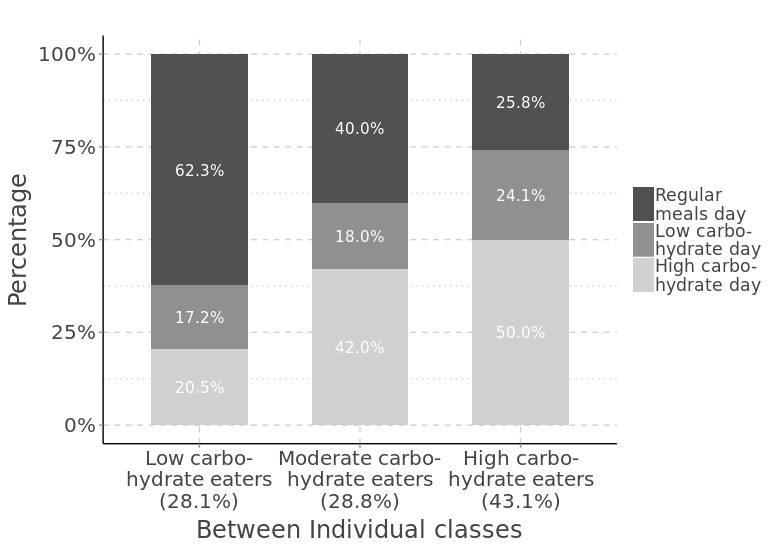
\includegraphics[width=27cm]{Fig/level2.png}	\vskip-2.45ex
	\caption{Multilevel Latent Class Solution, 3 classes in day level, 3 classes in individual level.}
\end{figure}


%    Class aptent taciti sociosqu ad litora torquent per conubia nostra, per
%    inceptos himenaeos. Phasellus libero enim, gravida sed erat sit amet,
%    scelerisque congue diam. Fusce dapibus dui ut augue pulvinar iaculis.
%
%    \begin{table}
%      \centering
%      \begin{tabular}{l r r c}
%        \toprule
%        \textbf{First column} & \textbf{Second column} & \textbf{Third column} & \textbf{Fourth} \\
%        \midrule
%        Foo & 13.37 & 384,394 & \alpha \\
%        Bar & 2.17 & 1,392 & \beta \\
%        Baz & 3.14 & 83,742 & \delta \\
%        Qux & 7.59 & 974 & \gamma \\
%        \bottomrule
%      \end{tabular}
%      \caption{A table caption.}
%    \end{table}
%
%    Donec quis posuere ligula. Nunc feugiat elit a mi malesuada consequat. Sed
%    imperdiet augue ac nibh aliquet tristique. Aenean eu tortor vulputate,
%    eleifend lorem in, dictum urna. Proin auctor ante in augue tincidunt
%    tempor. Proin pellentesque vulputate odio, ac gravida nulla posuere
%    efficitur. Aenean at velit vel dolor blandit molestie. Mauris laoreet
%    commodo quam, non luctus nibh ullamcorper in. Class aptent taciti sociosqu
%    ad litora torquent per conubia nostra, per inceptos himenaeos.
%
%    Nulla varius finibus volutpat. Mauris molestie lorem tincidunt, iaculis
%    libero at, gravida ante. Phasellus at felis eu neque suscipit suscipit.
%    Integer ullamcorper, dui nec pretium ornare, urna dolor consequat libero,
%    in feugiat elit lorem euismod lacus. Pellentesque sit amet dolor mollis,
%    auctor urna non, tempus sem.

  \end{block}

  \begin{block}{References}
    \vskip-1.25ex
%    \nocite{*}
    \footnotesize{\bibliographystyle{elsarticle-num}\bibliography{poster}}

  \end{block}

\end{column}

\separatorcolumn
\end{columns}
\end{frame}

\end{document}
